\chapter{Storage Benchmark Programs}
\label{BENCH}

%%The reason storage benchmarking is difficult and what we want to do.
Storage system performance is one of the most critical factors in meeting overall system performance expectations. 
The performance variances of typical storage systems today can vary by orders of magnitude~\cite{chen:1993}. 
It is very easy to get misled by the performance numbers without understanding the relationship between the storage workload and its performance variances. 

Characterizing the workload for storage systems is typically much more complex than it is for the processors. 
In a simple uni-processor case, it is possible to calculate metrics such as instruction per cycle based on the various cache misses, mis-predictions and number of instructions. 
However, storage systems typically have a much more state-dependent responses. 
For example, a cache miss does not always result in the same penalty, and the service time for a given request depends not only on the  current request but also on all requests in the queue as well as the layout of the data. 
Therefore, two very similar workloads may perform very differently since the small differences could force the state transition path into completely different directions. 
For example, current layout of the data could force a sequential write to become fragmented. 
This then cause the sequential read of the same data to be slow. 
This in turn has effect on any requests that are scheduled after it within the request buffer.

We evaluated current storage benchmarking tools and analyze the effects of different parameter settings on various performance metrics. 
Based on the experiments, we quantify the effects of various parameters for three benchmarks. 
In addition, we also evaluate which parameters are needed to effectively cover the entire storage system performance space and we propose a new benchmark tool based on our evaluation.

\section{Limitations of Current Approach}
The best method for benchmarking a storage system would be to deploy the system under test in the real environment and look at the execution time of the processes that will be run. 
Obviously this approach is too costly to evaluate various feature and performance enhancements. 
Therefore, system architects and designers resort to either a set of traces collected from a real system or a set of synthetic benchmarks.

The problem with using a real trace is that there is no way to determine the coverage of the workload space. 
For example, a given Exchange server trace may perform very well on system A. 
However, it is difficult to determine if system A will perform as well for all Exchange servers. 
Furthermore, it is impossible even to provide any range of potential performances with a single trace. 
As mentioned above, a small change in the trace could result in a very different performance results.

Numerous synthetic benchmarks have been proposed over last few decades. 
The major benefit of these benchmarks is that they allow you to change the characteristics of the workload in a quantitative manner. 
However, current benchmarks either provide numerous parameters to set without providing any insights to the importance of each parameter~\cite{axboe:2008, vandenbergh:2008, katcher:1997, wolman:1989, norcott:2006, coker:2001} or they provide a representative set of parameters that claim to represent a wide range of applications. 
When there are numerous parameters to set, users typically test a few set of ad hoc settings based on their experience which does not always  result in an accurate representation of real workloads. 

\section{Benchmark Programs under Test}
As a proof of concept, we evaluate two different benchmarks tools, PostMark~\cite{katcher:1997} and FIO~\cite{axboe:2008}.

Typically, the evaluated systems are only tested on single configuration of a given benchmark. 
This is problematic since system A may perform better than system B for one configuration of the benchmark but not the others. 
It is critical to either define when the system A performs better or show that system A performs better B in wide range of workloads by testing with multiple configurations that provide wide coverage. 

\subsection{PostMark}
\begin{table}
\centering
\begin{tabularx}{0.9\textwidth}{
  X | 
  >{\centering}X 
  >{\centering\arraybackslash}X
}
\hline
\bfseries Name        &\bfseries Level Low  &\bfseries Level High     \\
\hline\hline
min\_file\_size       &512B                 &4KiB                     \\
max\_file\_size       &4KiB                 &16MiB                    \\
init\_file\_count     &1000                 &10000                    \\
transaction\_count    &10000                &100000                   \\
read\_size            &512B                 &32KiB                    \\
write\_size           &512B                 &32KiB                    \\
file\_system\_buffer  &false                &true                     \\
read\_append\_ratio   &1:9                  &9:1                      \\
create\_delete\_ratio &5:5                  &9:1                      \\
directory\_count      &1                    &1000                     \\
\hline
\end{tabularx}
\captionsetup{format=myformat}
\caption{PostMark input parameters and input levels assigned to each parameter.}
\label{pm_param_t}
\end{table}
  
PostMark was designed for filesystem benchmarking with specific interest to performance of handling small file accesses in Internet software~\cite{katcher:1997}. 
It provides 10 different parameter settings shown in \tablename~\ref{pm_param_t} together with their level settings. 
Most of level decisions were straight forward except the \emph{create\_delete\_ratio}. 
Initially, we set the low bound to be 1:9 where 10\% of the operations are create and 90\% deletion. 
However, we soon realized that the bound is too unrealistic. 
If the deletion of file happens more than the creation, the system will soon become empty of files. 
Therefore, we set the low bound to be 50\% where the creation and deletion is equally like to occur. 

Aside from these, it also provide two more benchmarking parameter for setting the random variable seed and controlling result format. 
The \emph{transaction\_count} only controls the duration of the run and not the arrival rate or the IO depth. 
Therefore, it is also a benchmark parameter. 
The \emph{file\_system\_buffer} parameter is a system parameter which is forces all writes to bypass the filesystem buffer.

PostMark lacks control over arrival pattern and does not support sequential access pattern. 
Since these two characteristics play a major role in how the storage system performs, we can guess that the coverage of PostMark will not be great. 
Also, Postmark does not perform any overwrites which suggest that Postmark is unsuitable for evaluating storage systems where overwrites are expensive such as SSDs.
 
Postmark reports seven performance metrics, \emph{transaction per second} (tps), create tps, read tps, append tps, delete tps, read throughput and write throughput. 
 
\subsection{Flexible IO Tester (FIO)}
\begin{table}
\centering
\begin{tabularx}{0.9\textwidth}{
  X | 
  >{\centering}X 
  >{\centering\arraybackslash}X
}
\hline
\bfseries Name      &\bfseries Level Low  &\bfseries Level High     \\
\hline\hline
operation           &read                 &write                    \\
access\_pattern     &sequential           &random                   \\
files\_used         &1                    &100                      \\
min\_file\_size     &512B                 &1MiB                     \\
max\_file\_size     &1MiB                 &1GiB                     \\
min\_block\_size    &512                  &4KiB                     \\
max\_block\_size    &4KiB                 &64KiB                    \\
io\_depth           &1                    &100                      \\
overwrite           &false                &true                     \\
fsync               &false                &true                     \\
thinktime           &0us                  &1000us                   \\
write\_buffer\_sync &false                &true                     \\
file\_service       &roundrobin           &random                   \\
thread\_count       &1                    &8                        \\
threads\_similarity &false                &true                     \\
posix\_fadvise      &false                &true                     \\
async\_io\_engine   &false                &true                     \\
io\_engine\_queue   &false                &true                     \\
directio            &false                &true                     \\
buffer\_alloc       &malloc               &mmap                     \\
\hline
\end{tabularx}
\captionsetup{format=myformat}
\caption{FIO input parameters and input levels assigned to each parameter.}
\label{fio_param_t}
\end{table}

FIO was designed for benchmarking as well as stress/hardware verification~\cite{axboe:2008}. 
It works directly on block devices as well as files. 
In this experiment, we tested it on files for the sake of consistency with PostMark.

FIO has over 30 different input parameters. 
However, some of those parameters are completely dependent on other parameters and was discarded. 
Also, some of the parameters, when set, caused bus errors on the system we tested. 
As a result, we extracted 20 input parameters as shown in \tablename~\ref{fio_param_t}. 
Every experiment was run for 10 minutes., which was sufficient to ensure that the system reached a steady state. 

FIO can generate multiple independent streams of requests. 
In this study, we evaluate the effect of multiple streams as function of two parameters, \emph{thread\_count} and \emph{threads\_similarity}. 
The thread\_count parameter is self-explanatory. 
When the thread\_similarity is true, we generate either set of very similar streams with only difference being the random seed. 
When it is false, we generate threads that are at maximum distances from each other in the parameter space. 
This can be achieved by choosing different experiments within PB design.

FIO also allows you to control number of outstanding requests controlled by \emph{io\_depth}. 
The \emph{posix\_fadvise} option allows to you enable file advisory information to the operating system~\cite{plonka:2007}. 
FIO provides 13 different types of IO engines. 
Some of them did not work on our system but we use 4 based on the two characteristics of the IO engines, synchronous/asynchronous and multiple/single buffer.

FIO provides a detailed distribution of performance measurements as well as aggregated numbers. 
In our study, we use 4 metrics, read throughput, write throughput, average read latency and average write latency. 
These metrics were chosen not only because they are important performance metrics but also so that the results can be compared against PostMark for out coverage analysis. 
For the experiments with more than 1 thread, the throughputs are simply added and the latency is averaged.

\section{Quantative Analysis}

\subsection{Experiment Flow}
 The experiment is designed to evaluate the effect of various parameters of different benchmarks and coverage of each benchmark. 
We first use PB design to evaluate the effect of each parameter with minimum number of experiments.  
Once the effect has been calculated, we perform ICA on the performance results from each benchmark to estimate equal number of independent components. 
These components are clustered to generate a view of coverage of each benchmark.
 
 This lets us analyze what are the key parameters and whether both benchmarks are needed for a through evaluation of storage systems.

\subsubsection{Evaluation of Benchmark Parameter Effect}

\begin{figure}[!t]
\centering
\begin{tikzpicture}[auto,node distance=2cm]
    % Place nodes
    \node [block, node distance=4cm] (init) {Parameter Extraction};
    \node [cloud, left of=init, node distance=6cm] (manual) {Benchmark Manual};
    \node [block, below of=init] (lvl) {Parameter Level Decision};
    \node [block, below of=manual] (PB) {PB Experiment Generation};
    \node [cloud, below of=lvl] (p_list) {Parameter List};
    \node [cloud, below of=PB] (PB_table) {PB Table};
    \node [block, below of=p_list] (input) {Benchmark Input Parameter Generation};
    \node [block, left of=input, node distance=6cm] (run) {Run Benchmarks};
    \node [cloud, below of=run](result){Results};
    \node [block, right of=result, node distance = 6cm](eval){Effect Estimation};
    % Draw edges
    \path [line] (manual) -- (init);
    \path [line] (init) -- (lvl);
    \path [line] (init) -- (PB);
    \path [line] (PB) -- (PB_table);
    \path [line] (lvl) -- (p_list);
    \path [line] (p_list) -- (input);
    \path [line] (PB_table) -- (input);
    \path [line] (input) -- (run);
    \path [line] (run) -- (result);
    \path [line] (result) -- (eval);
    \path [line] (input) -- (eval);
\end{tikzpicture}

\captionsetup{format=myformat}
\caption{Experiment flow for estimating the parameter effects on performance.}
\label{pb_flow_t}
\end{figure}

First, we use PB method to determine the effect of each parameters on each benchmarks seperately. 
The experiment flow for effect estimation is shown in \figurename~\ref{pb_flow_t}. 
\emph{Parameter Extraction} phase tries to extract parameters from benchmark documentation in such a way that each parameter can be varied independently of others. 
This is not always easy as shown in the description of the benchmarks. 

For every parameter extracted, a two extreme level values are designated as shown in \tablename~\ref{pm_param_t} and \tablename~\ref{fio_param_t}. 
Also, once the number of parameter is known, the size of PB design is also known which is required to generate PB design table.  
Since the number of parameters for Postmark is 10 and FIO is 22, PB table of size 12 and 24 are used respectively. 
While any Hardamard matrix~\cite{hadamar:1954} can be used, we use the matrices shown in equation \ref {pb12} for 11 factor experiment.  
PB table for 23 factors can be found in Plackett and Burman's original paper~\cite{plackett:1946} and we omit it due to the space constraint. 

\begin{equation}\label{pb12}
\mathbf{PB}(12)=
\left [ {\begin{array}{r r r r r r r r r r r}
  1&  1& -1&  1&  1&  1& -1& -1& -1&  1& -1\\
 -1&  1&  1& -1&  1&  1&  1& -1& -1& -1&  1\\
  1& -1&  1&  1& -1&  1&  1&  1& -1& -1& -1\\
 -1&  1& -1&  1&  1& -1&  1&  1&  1& -1& -1\\
 -1& -1&  1& -1&  1&  1& -1&  1&  1&  1& -1\\
 -1& -1& -1&  1& -1&  1&  1& -1&  1&  1&  1\\
  1& -1& -1& -1&  1& -1&  1&  1& -1&  1&  1\\
  1&  1& -1& -1& -1&  1& -1&  1&  1& -1&  1\\
  1&  1&  1& -1& -1& -1&  1& -1&  1&  1& -1\\
 -1&  1&  1&  1& -1& -1& -1&  1& -1&  1&  1\\
  1& -1&  1&  1&  1& -1& -1& -1&  1& -1&  1\\
 -1& -1& -1& -1& -1& -1& -1& -1& -1& -1& -1\\
\end{array}} \right ] 
\end{equation}

Each row of the PB table represents an experiment and columns represent parameters. 
$-1$ value represents a \emph{low level} while $1$ represents a \emph{high level}. 
It should be noted that not every column can be assigned a parameter. 
You can leave any of the columns out for actual run of the experiments. 
However, it is important to ignore the effect of the unused column later. 

The number of experiment required in equivalent to the number of row of the matrix. 
Every experiment is repeated three times and mean is used to calculate the effect. 
Given $n$ experiment result $\mathbf{y}$, the effect, $e$, of a parameter represented by column $i$ of PB matrix is simply calculated by
\begin{equation}
e=\frac{\mathbf{PB}_i \cdot \mathbf{y}}{\sum \limits_i (\mathbf{PB}_i \cdot \mathbf{y})}.
\end{equation}
Here the denominator is a simple normalization factor to ensure that sum of all effects is 1. 

\subsubsection{Evaluations of Benchmark Coverage}

We use R JADE package~\cite{ilmonen:2010} to generate 2, 4, 8 independent components from the input parameters and the read and the write throughput measured from each benchmark. 
Since the read and the write throughputs are the only common metrics reported from the two benchmarks, only they can be directly compared. 

Once components are estimated, we evaluate the Euclidean distances between all components which corresponds to a single performance metric are calculated. 
Based on the distance, the components are clustered. 
The number of clusters to be used were estimated using dendrograms~\cite{szekely:2005}. 

We evaluate the best number of components for clean clustering and determine the coverage of each benchmark on two performance metrics.  

\section{Results}

\subsection{Effects}
\begin{figure}[!t]
\centering
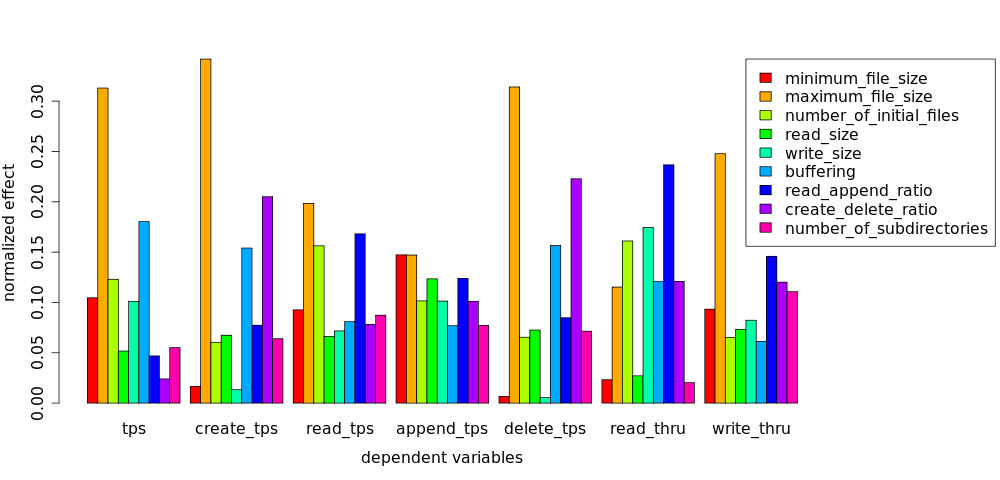
\includegraphics[width=0.9\textwidth]{figure/pm_effect.png}
\captionsetup{format=myformat}
\caption{PostMark parameter effects. 
You can see that some parameters have high effect on a particular kind of performance matric while some have high effect on almost all performance matrics.}
\label{pm_effect}
\end{figure}

\begin{figure}[!t]
\centering
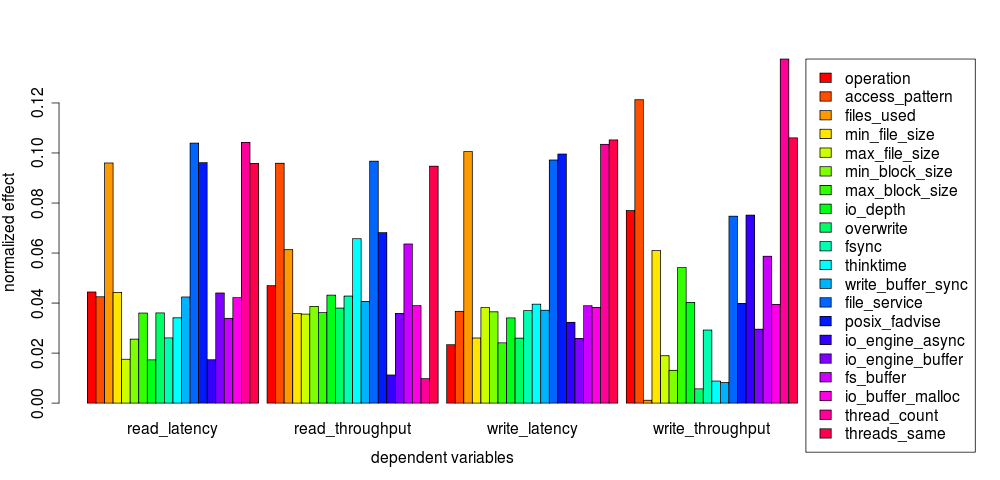
\includegraphics[width=0.9\textwidth]{figure/fio_effect.png}
\captionsetup{format=myformat}
\caption{FIO parameter effects. 
Effect of application threading is the most pronounced in this bechmark. 
However, it will be shown later that the effect of threading can be triggered by other paramters as well.}
\label{fio_effect}
\end{figure}

\figurename~\ref{pm_effect} shows effect of each parameter on each performance metrics reported by Postmark. 
The \emph{maximum\_file\_ size} and \emph{buffering} are the clearly two most important factor in deciding the overall tps. 
The \emph{buffering} parameter controls whether file system buffer should be bypassed using direct IO and the importance of the parameter is obvious. 
However, the effect of the \emph{maximum\_file\_ size} is less obvious. 
Potentially, the high effect is due to the fact that larger file sizes allow a room for longer sequential accesses while the small file sizes force overall access pattern to behave in a more random fashion. 

You can also see that different performance metrics are effected differently. 
The \emph{create\_delete\_ratio} is clearly and obviously important for create tps and delete tps while for append tps, file sizes are more important. 
Another interesting to note is that while read throughput is affected the most by the \emph{read\_append\_ratio}, the write throughput is much more impacted by the file size.

Table \ref{pm_50_t} shows list of parameters with the most effect on each performance metric such that sum of the effects exceed 50\%of overall effects. 
It is shown that roughly 50\% of the all performance variances can be captured using just 2-4 parameters. 
For example, three parameters, \emph{maximum\_file\_size}, \emph{number\_of\_initial\_files} and \emph{buffering}, contribute to 61\% of overall tps variation observed. 
This equate to 4 to 16 experiments for exhaustive evaluation. 
This is a huge improvements over 2048 experiments required for original 12 parameters. 
Furthermore, it is clear that different input combinations must be tested for each performance metric which must be taken into consideration when benchmarking storage systems. 

\begin{table}[!t]
\centering
\begin{tabularx}{0.9\textwidth}{
  l | 
  X 
  c
}
\hline
\bfseries Performance Metric   &\bfseries Parameters           &\bfseries Total Effect  \\
\hline\hline
tps           & maximum\_file\_size                             &0.6164   \\
              & number\_of\_initial\_files                      &         \\
              & filesystem\_buffer                              &         \\
\hline
create\_tps   & maximum\_file\_size                             &0.5469   \\
              & create\_delete\_ratio                           &         \\
\hline
read\_tps     & maximum\_file\_size                             &0.5229   \\
              & number\_of\_initial\_files                      &         \\
              & read\_append\_ratio                             &         \\
\hline
append\_tps   & minimum\_file\_size                             &0.5418   \\
              & maximum\_file\_size                             &         \\
              & read\_size                                      &         \\
              & read\_append\_ratio                             &         \\
\hline
delete\_tps   & maximum\_file\_size                             &0.5369   \\
              & create\_append\_ratio                           &         \\
\hline
read\_thru    & number\_of\_initial\_files                      &0.5722   \\
              & write\_size                                     &         \\
              & read\_append\_ratio                             &         \\
\hline
write\_thru   & maximum\_file\_size                             &0.5137   \\
              & read\_append\_ratio                             &         \\
              & create\_delete\_ratio                           &         \\
\hline
\end{tabularx}
\captionsetup{format=myformat}
\caption{PostMark input parameters required to cover at least 50\% of overall effect for each performance metrics reported.
The maximum number of parameters required does not exceed 4.}
\label{pm_50_t}
\end{table}

\begin{table}[!t]
\centering
\begin{tabularx}{0.9\textwidth}{
  l | 
  X 
  c
}
\hline
\bfseries Performance Metric &\bfseries Parameters &\bfseries Total Effect\\
\hline\hline
read\_latency       & files\_used                               &0.5406   \\
                    & file\_service                             &         \\ 
                    & posix\_fadvise                            &         \\ 
                    & thread\_count                             &         \\
                    & threads\_same                             &         \\
\hline
read\_throughput    & access\_pattern                           &0.5462   \\
                    & write\_buffer\_sync                       &         \\
                    & threads\_same                             &         \\
\hline
write\_latency      & files\_used                               &0.5060   \\
                    & file\_service                             &         \\
                    & posix\_fadvise                            &         \\
                    & thread\_count                             &         \\
                    & threads\_same                             &         \\
\hline
write\_throughput   & access\_pattern                           &0.5170   \\  
                    & thread\_count                             &         \\ 
                    & threads\_same                             &         \\
\hline
\end{tabularx}
\captionsetup{format=myformat}
\caption{FIO input parameters required to cover at least 50\% of overall effect of each performance metrics reported.
The maximum number of parameters required does not exceed 5.}
\label{fio_50_t}
\end{table}

\figurename~\ref{fio_effect} shows the effect of each parameter on four performance metrics measured and \tablename~\ref{fio_50_t} shows list of parameters with the most effect on each performance metric such that sum of the effects exceed 50\%of overall effects. It is interesting to note that the most important parameters for read and write latencies are the same. We can assume that read and write operations themselves do not affect the latency in our system. This can expected, since on HDD, read and write operations do not result in significantly different response time.  Furthermore, we see that the \emph{threads\_same} parameter is important for all metrics. This indicates that the interference between the threads can seriously affect the performance. While the \emph{thread\_count} parameter is also important, the effect on the read throughput is shown to be negligible. Both throughputs are sensitive to the \emph{access\_pattern} which is expected but surprisingly the latency is not. Instead, they are much more sensitive to the \emph{posix\_fadvise} setting. This suggests that latency is not determined by the seek time but rather cache miss penalties. 

\subsection{Coverage of Benchmarks}


\begin{figure}[!t]
\centering
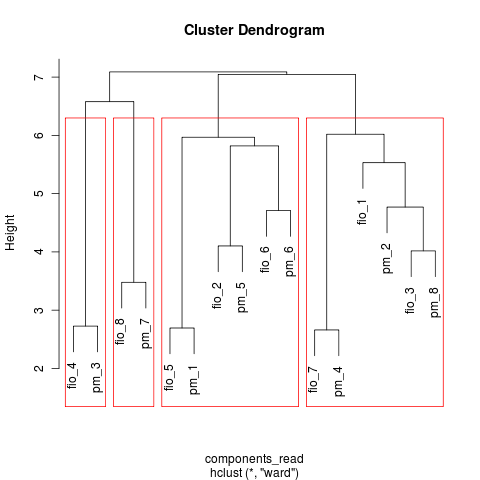
\includegraphics[width=0.8\textwidth]{figure/Rplot001.png}
\captionsetup{format=myformat}
\caption{Read performance coverage of of independent components of PostMark and FIO.}
\label{read_cov}
\end{figure}

\begin{figure}[!t]
\centering
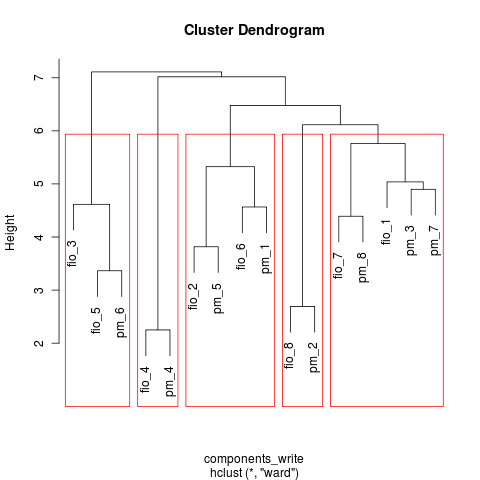
\includegraphics[width=0.8\textwidth]{figure/Rplot002.png}
\captionsetup{format=myformat}
\caption{Write performance coverage of of independent components of PostMark and FIO.}
\label{write_cov}
\end{figure}

The distance between the independent components as well as their clustering is shown in \figurename~\ref{read_cov} and \figurename~\ref{write_cov}. 
In these graphs, each leaf node represents an independent component. 
Since the independent components have no physical meaning associated with them, we number them from 1 to 8 per benchmark. 
We only show the results of 8 components for the brevity. The closer the leaves are on the tree, more similar effect they have on the result. The \emph{height} represents the difference between the subtrees. therefore, evenly spread out components of both benchmark on x-axis suggest similar coverage, while the height of the tree suggest the granularity of the coverage. For example, the FIO component 4 and PostMark component 3 have the similar effect on the read throughput based on the \figurename~\ref{read_cov}. At the same time, FIO component 8 and PostMark component 7 also have similar effect. However, there is a large gap between the two sets of components which are not covered by any of the components as suggested by the \emph{height} of the edges connecting the two subtrees.

An interesting observation is that for read throughput, FIO and Postmark have roughly the same coverage. This is interesting since PostMark have far fewer parameters. It can be concluded if the metric of interest is read throughput, than it does not matter which benchmark you use as long as you can test the key parameters thoroughly.

For the write throughput, FIO does provide wider coverage to the left with component 3, while PostMark provide wider coverage on the right with component 3 and 7. We can safely conclude that each benchmark provide one of more input parameters that affect the write throughput that is not provided by the other benchmark. 

The input parameters that affect the read and write throughput performance shows some difference. They all depend on the size of the files, number of files and mix of operations. However, write throughput is also dependent on file creation and deletion which are not taken into account in FIO. Conversely, PostMark does not consider the number of threads which is another important factor provided by FIO. 

We believe that a good benchmark should have all those components as inputs to provide a wider coverage. 

\section{Conclusion}
Clearly, any storage performance evaluation should consider the effect of critical input parameters that has been described in this paper. We recommend that at least the critical parameters shown in \tablename~\ref{pm_50_t} and \ref{fio_50_t} should be tested thoroughly to gain an approximate sense of the system's performance variation.

The methodology presented in this paper can be applied to any benchmarking tool with set of input parameters that can be adjusted. The key challenge is deciding the range of each parameter. Once this is done, the entire process can be automated. 

Even if the system is designed for a specific workload, it is still beneficial to follow the methodology described in this paper. Since the characteristics of the actual workload is known, a tighter level bounds can be assigned to each parameter. The resulting effect of the parameters can describe how the system reacts to different parameters and can provide valuable insights to workload-system interactions. 

We also show that different benchmarks can still cover roughly the same performance space if the input parameters are chosen appropriately. We suggest that performing a set of through experiments on a single benchmark provides more accurate description of system performance than running a single experiment on the multiple benchmarks. 

However, it is clear that there are specific performance space that can only be explored with a specific benchmark. Since it is difficult to determine what benchmarks cover how much of the performance space, we propose a new benchmark with following properties.
\begin{itemize}
\item IO benchmark tool should provide maximum coverage of storage system's operational space with minimum parameter settings.  
\item The parameters of benchmarking tools should be as independent as possible.
\item The parameters should be exclusively defined as either the system parameter, the workload parameter or the benchmark parameter. 
\item The target interface which the benchmark is testing needs to be clearly defined. 
\item A minimum validation of results should be handled. (eg. Results that suggest under-utilization of target system such that the performance result does reflect its capability.)
\end{itemize}

With this kind of benchmarking tool, most of the systems can be evaluated with a single benchmark with multiple parameter settings. This tool would allow different researcher and developers to report their performance in a more coherent manner which in turn makes performance comparison and reproducing the result easier. 

As a future work, we plan to conduct a comprehensive analysis of more benchmarks and design a new benchmark that provides a wide coverage with few independent parameters. 

